% Options for packages loaded elsewhere
\PassOptionsToPackage{unicode}{hyperref}
\PassOptionsToPackage{hyphens}{url}
\PassOptionsToPackage{dvipsnames,svgnames,x11names}{xcolor}
%
\documentclass[
  letterpaper,
  DIV=11,
  numbers=noendperiod]{scrreprt}

\usepackage{amsmath,amssymb}
\usepackage{iftex}
\ifPDFTeX
  \usepackage[T1]{fontenc}
  \usepackage[utf8]{inputenc}
  \usepackage{textcomp} % provide euro and other symbols
\else % if luatex or xetex
  \usepackage{unicode-math}
  \defaultfontfeatures{Scale=MatchLowercase}
  \defaultfontfeatures[\rmfamily]{Ligatures=TeX,Scale=1}
\fi
\usepackage{lmodern}
\ifPDFTeX\else  
    % xetex/luatex font selection
  \setmainfont[]{Times New Roman}
\fi
% Use upquote if available, for straight quotes in verbatim environments
\IfFileExists{upquote.sty}{\usepackage{upquote}}{}
\IfFileExists{microtype.sty}{% use microtype if available
  \usepackage[]{microtype}
  \UseMicrotypeSet[protrusion]{basicmath} % disable protrusion for tt fonts
}{}
\makeatletter
\@ifundefined{KOMAClassName}{% if non-KOMA class
  \IfFileExists{parskip.sty}{%
    \usepackage{parskip}
  }{% else
    \setlength{\parindent}{0pt}
    \setlength{\parskip}{6pt plus 2pt minus 1pt}}
}{% if KOMA class
  \KOMAoptions{parskip=half}}
\makeatother
\usepackage{xcolor}
\setlength{\emergencystretch}{3em} % prevent overfull lines
\setcounter{secnumdepth}{5}
% Make \paragraph and \subparagraph free-standing
\ifx\paragraph\undefined\else
  \let\oldparagraph\paragraph
  \renewcommand{\paragraph}[1]{\oldparagraph{#1}\mbox{}}
\fi
\ifx\subparagraph\undefined\else
  \let\oldsubparagraph\subparagraph
  \renewcommand{\subparagraph}[1]{\oldsubparagraph{#1}\mbox{}}
\fi

\usepackage{color}
\usepackage{fancyvrb}
\newcommand{\VerbBar}{|}
\newcommand{\VERB}{\Verb[commandchars=\\\{\}]}
\DefineVerbatimEnvironment{Highlighting}{Verbatim}{commandchars=\\\{\}}
% Add ',fontsize=\small' for more characters per line
\usepackage{framed}
\definecolor{shadecolor}{RGB}{241,243,245}
\newenvironment{Shaded}{\begin{snugshade}}{\end{snugshade}}
\newcommand{\AlertTok}[1]{\textcolor[rgb]{0.68,0.00,0.00}{#1}}
\newcommand{\AnnotationTok}[1]{\textcolor[rgb]{0.37,0.37,0.37}{#1}}
\newcommand{\AttributeTok}[1]{\textcolor[rgb]{0.40,0.45,0.13}{#1}}
\newcommand{\BaseNTok}[1]{\textcolor[rgb]{0.68,0.00,0.00}{#1}}
\newcommand{\BuiltInTok}[1]{\textcolor[rgb]{0.00,0.23,0.31}{#1}}
\newcommand{\CharTok}[1]{\textcolor[rgb]{0.13,0.47,0.30}{#1}}
\newcommand{\CommentTok}[1]{\textcolor[rgb]{0.37,0.37,0.37}{#1}}
\newcommand{\CommentVarTok}[1]{\textcolor[rgb]{0.37,0.37,0.37}{\textit{#1}}}
\newcommand{\ConstantTok}[1]{\textcolor[rgb]{0.56,0.35,0.01}{#1}}
\newcommand{\ControlFlowTok}[1]{\textcolor[rgb]{0.00,0.23,0.31}{#1}}
\newcommand{\DataTypeTok}[1]{\textcolor[rgb]{0.68,0.00,0.00}{#1}}
\newcommand{\DecValTok}[1]{\textcolor[rgb]{0.68,0.00,0.00}{#1}}
\newcommand{\DocumentationTok}[1]{\textcolor[rgb]{0.37,0.37,0.37}{\textit{#1}}}
\newcommand{\ErrorTok}[1]{\textcolor[rgb]{0.68,0.00,0.00}{#1}}
\newcommand{\ExtensionTok}[1]{\textcolor[rgb]{0.00,0.23,0.31}{#1}}
\newcommand{\FloatTok}[1]{\textcolor[rgb]{0.68,0.00,0.00}{#1}}
\newcommand{\FunctionTok}[1]{\textcolor[rgb]{0.28,0.35,0.67}{#1}}
\newcommand{\ImportTok}[1]{\textcolor[rgb]{0.00,0.46,0.62}{#1}}
\newcommand{\InformationTok}[1]{\textcolor[rgb]{0.37,0.37,0.37}{#1}}
\newcommand{\KeywordTok}[1]{\textcolor[rgb]{0.00,0.23,0.31}{#1}}
\newcommand{\NormalTok}[1]{\textcolor[rgb]{0.00,0.23,0.31}{#1}}
\newcommand{\OperatorTok}[1]{\textcolor[rgb]{0.37,0.37,0.37}{#1}}
\newcommand{\OtherTok}[1]{\textcolor[rgb]{0.00,0.23,0.31}{#1}}
\newcommand{\PreprocessorTok}[1]{\textcolor[rgb]{0.68,0.00,0.00}{#1}}
\newcommand{\RegionMarkerTok}[1]{\textcolor[rgb]{0.00,0.23,0.31}{#1}}
\newcommand{\SpecialCharTok}[1]{\textcolor[rgb]{0.37,0.37,0.37}{#1}}
\newcommand{\SpecialStringTok}[1]{\textcolor[rgb]{0.13,0.47,0.30}{#1}}
\newcommand{\StringTok}[1]{\textcolor[rgb]{0.13,0.47,0.30}{#1}}
\newcommand{\VariableTok}[1]{\textcolor[rgb]{0.07,0.07,0.07}{#1}}
\newcommand{\VerbatimStringTok}[1]{\textcolor[rgb]{0.13,0.47,0.30}{#1}}
\newcommand{\WarningTok}[1]{\textcolor[rgb]{0.37,0.37,0.37}{\textit{#1}}}

\providecommand{\tightlist}{%
  \setlength{\itemsep}{0pt}\setlength{\parskip}{0pt}}\usepackage{longtable,booktabs,array}
\usepackage{calc} % for calculating minipage widths
% Correct order of tables after \paragraph or \subparagraph
\usepackage{etoolbox}
\makeatletter
\patchcmd\longtable{\par}{\if@noskipsec\mbox{}\fi\par}{}{}
\makeatother
% Allow footnotes in longtable head/foot
\IfFileExists{footnotehyper.sty}{\usepackage{footnotehyper}}{\usepackage{footnote}}
\makesavenoteenv{longtable}
\usepackage{graphicx}
\makeatletter
\def\maxwidth{\ifdim\Gin@nat@width>\linewidth\linewidth\else\Gin@nat@width\fi}
\def\maxheight{\ifdim\Gin@nat@height>\textheight\textheight\else\Gin@nat@height\fi}
\makeatother
% Scale images if necessary, so that they will not overflow the page
% margins by default, and it is still possible to overwrite the defaults
% using explicit options in \includegraphics[width, height, ...]{}
\setkeys{Gin}{width=\maxwidth,height=\maxheight,keepaspectratio}
% Set default figure placement to htbp
\makeatletter
\def\fps@figure{htbp}
\makeatother

\KOMAoption{captions}{tableheading}
\makeatletter
\makeatother
\makeatletter
\@ifpackageloaded{bookmark}{}{\usepackage{bookmark}}
\makeatother
\makeatletter
\@ifpackageloaded{caption}{}{\usepackage{caption}}
\AtBeginDocument{%
\ifdefined\contentsname
  \renewcommand*\contentsname{Содержание}
\else
  \newcommand\contentsname{Содержание}
\fi
\ifdefined\listfigurename
  \renewcommand*\listfigurename{Список Иллюстраций}
\else
  \newcommand\listfigurename{Список Иллюстраций}
\fi
\ifdefined\listtablename
  \renewcommand*\listtablename{Список Таблиц}
\else
  \newcommand\listtablename{Список Таблиц}
\fi
\ifdefined\figurename
  \renewcommand*\figurename{Рисунок}
\else
  \newcommand\figurename{Рисунок}
\fi
\ifdefined\tablename
  \renewcommand*\tablename{Таблица}
\else
  \newcommand\tablename{Таблица}
\fi
}
\@ifpackageloaded{float}{}{\usepackage{float}}
\floatstyle{ruled}
\@ifundefined{c@chapter}{\newfloat{codelisting}{h}{lop}}{\newfloat{codelisting}{h}{lop}[chapter]}
\floatname{codelisting}{Список}
\newcommand*\listoflistings{\listof{codelisting}{Список Каталогов}}
\makeatother
\makeatletter
\@ifpackageloaded{caption}{}{\usepackage{caption}}
\@ifpackageloaded{subcaption}{}{\usepackage{subcaption}}
\makeatother
\makeatletter
\@ifpackageloaded{tcolorbox}{}{\usepackage[skins,breakable]{tcolorbox}}
\makeatother
\makeatletter
\@ifundefined{shadecolor}{\definecolor{shadecolor}{rgb}{.97, .97, .97}}
\makeatother
\makeatletter
\makeatother
\makeatletter
\makeatother
\ifLuaTeX
\usepackage[bidi=basic]{babel}
\else
\usepackage[bidi=default]{babel}
\fi
\babelprovide[main,import]{russian}
% get rid of language-specific shorthands (see #6817):
\let\LanguageShortHands\languageshorthands
\def\languageshorthands#1{}
\ifLuaTeX
  \usepackage{selnolig}  % disable illegal ligatures
\fi
\IfFileExists{bookmark.sty}{\usepackage{bookmark}}{\usepackage{hyperref}}
\IfFileExists{xurl.sty}{\usepackage{xurl}}{} % add URL line breaks if available
\urlstyle{same} % disable monospaced font for URLs
\hypersetup{
  pdftitle={R в социологических исследованиях},
  pdfauthor={Дарья Омельченко},
  pdflang={ru},
  colorlinks=true,
  linkcolor={blue},
  filecolor={Maroon},
  citecolor={Blue},
  urlcolor={Blue},
  pdfcreator={LaTeX via pandoc}}

\title{R в социологических исследованиях}
\author{Дарья Омельченко}
\date{}

\begin{document}
\maketitle
\ifdefined\Shaded\renewenvironment{Shaded}{\begin{tcolorbox}[borderline west={3pt}{0pt}{shadecolor}, interior hidden, sharp corners, frame hidden, boxrule=0pt, enhanced, breakable]}{\end{tcolorbox}}\fi

\renewcommand*\contentsname{Содержание}
{
\hypersetup{linkcolor=}
\setcounter{tocdepth}{2}
\tableofcontents
}
\bookmarksetup{startatroot}

\hypertarget{ux432-ux43aux430ux447ux435ux441ux442ux432ux435-ux43fux440ux435ux434ux438ux441ux43bux43eux432ux438ux44f}{%
\chapter*{В качестве
предисловия\ldots{}}\label{ux432-ux43aux430ux447ux435ux441ux442ux432ux435-ux43fux440ux435ux434ux438ux441ux43bux43eux432ux438ux44f}}
\addcontentsline{toc}{chapter}{В качестве предисловия\ldots{}}

\markboth{В качестве предисловия\ldots{}}{В качестве
предисловия\ldots{}}

Это электронное пособие написано для магистрантов, обучающихся по
направлению\ldots{}

\bookmarksetup{startatroot}

\hypertarget{ux43eux441ux43dux43eux432ux43dux44bux435-ux441ux432ux435ux434ux435ux43dux438ux44f-ux43eux431-r}{%
\chapter{Основные сведения об
R}\label{ux43eux441ux43dux43eux432ux43dux44bux435-ux441ux432ux435ux434ux435ux43dux438ux44f-ux43eux431-r}}

\hypertarget{ux447ux442ux43e-ux442ux430ux43aux43eux435-r}{%
\section{Что такое
R?}\label{ux447ux442ux43e-ux442ux430ux43aux43eux435-r}}

R -- это язык программирования и свободная программная среда для
статистической обработки и визуализации данных.

Несмотря на наличие огромного количества языков программирования и
различных программ для статистической обработки данных, R в течение двух
десятилетий остается популярным языком и средой обработки и анализа
данных для специалистов из разных областей знания.

Позиции языка R среди других языков программирования довольно высоки.
Так, по данным индекса Tiobe за 2022 год, R занимает 12-е место в мире:

\includegraphics{index_files/mediabag/tiobe.png}

Однако, прежде всего, это язык, который используют ученые, специалисты,
работающие в различных отраслях экономики, менеджеры для анализа
реальных данных и разработки научно обоснованных систем принятия
решений, поэтому место в общем рейтинге не так высоко. Если посмотреть
сферы использования, то на первом месте - академическая среда, на втором
- сфера здравоохранения, на третьем - правительственные учреждения.

\includegraphics{index_files/mediabag/4304a6e40e6cb86c9905.png}

R используют банки и маркетинговые агентства, технические компании и
информационные гиганты для разных целей - от обработки данных до
прогнозирования и представления интерактивной инфографики.

Вот только небольшой список тех компаний, которые используют R в своей
деятельности.

\includegraphics{https://gilesd-j.com/wp-content/uploads/2019/01/4-companies-using-R.jpg}

\hypertarget{ux43dux435ux43cux43dux43eux433ux43e-ux438ux441ux442ux43eux440ux438ux438}{%
\section{Немного
истории}\label{ux43dux435ux43cux43dux43eux433ux43e-ux438ux441ux442ux43eux440ux438ux438}}

R был создан профессорами \textbf{Россом Ихака} и \textbf{Робертом
Джентельменом} (Ross Ihaka и Robert Gentleman) в 1992 году, сначала как
язык программирования для обучения студентов статистике в университете
Окленда (Новая Зеландия). Авторы вдохновлялись при создании языком S,
используемым в лаборатории Bell, и ради шутки назвали язык R - по первым
буквам собственных имен.

В июне 1995 года, статистик \textbf{Мартин Махлер} убедил Ихаку и
Джентельмена опубликовать R как язык со свободным исходным кодом под
публичной лицензией GNU. Первая официальная версия была выпущена 29
февраля 2000 года.

Чуть ранее, в 1997 году \textbf{Куртом Хорником} и \textbf{Фрицем
Лейшем} была основана Сеть для архивирования кода R (CRAN, The
Comprehensive R Archive Network), цель которой заключалась в хранении
исходного кода, выполняемых файлов, документации и библиотек,
создаваемых пользователями. На момент декабря 2022 года CRAN имел 103
зеркальных сервера и 18 976 библиотек.

Команда разработчиков (R Core Team) также была основана в 1997 году для
дальнейшего развития языка. Сейчас в ней состоят ведующие разработчики,
статистики, специалисты по компьютерным наукам, всего более 20 человек.
В апреле 2003 года для развития проекта была создана некоммерческая
организация R Foundation. Цель фонда заключается в предоставлении
технической поддержки и коммуникации с создателями R, хранении и
управлении технической документацией и интеллектуальной собственностью.

Создатели R:

\textbf{Роберт Джентельмен}

\includegraphics{index_files/mediabag/200px-Rober_Gentlema.png}

\textbf{Росс Ихака}:

\includegraphics{index_files/mediabag/200px-Ross_Ihaka_-51.jpg}

\hypertarget{ux43aux430ux43aux43eux432ux44b-ux43fux440ux435ux438ux43cux443ux449ux435ux441ux442ux432ux430-r}{%
\section{Каковы преимущества
R?}\label{ux43aux430ux43aux43eux432ux44b-ux43fux440ux435ux438ux43cux443ux449ux435ux441ux442ux432ux430-r}}

Их довольно много:

\begin{enumerate}
\def\labelenumi{\arabic{enumi}.}
\tightlist
\item
  Возможности для \textbf{статистической обработки}, от простых функций
  до сложных моделей.
\end{enumerate}

Почти все новое, что появляется в области статистики, можно найти в
одной из библиотек R. Например, ANZ банк использует R для моделирования
невыплат по ипотечному кредитованию, а The Bank Of America применяет R
для формирования финансовой отчетности.

\begin{enumerate}
\def\labelenumi{\arabic{enumi}.}
\setcounter{enumi}{1}
\tightlist
\item
  Это язык программирования \textbf{с открытым исходным кодом}
  (Open-source)
\end{enumerate}

Что это значит? Это значит, что, во-первых, все написанное на R открыто
для изучения и критики, а, во-вторых, каждый может внести вклад в его
развитие и улучшение путем создания новых библиотек и новых функций для
решения различных задач.

\begin{enumerate}
\def\labelenumi{\arabic{enumi}.}
\setcounter{enumi}{2}
\tightlist
\item
  \textbf{Поддержка сообщества} (Community)
\end{enumerate}

У R - более 2 миллионов пользователей по всему миру, сообщество
пользователей R не только внушительное по размеру, но и очень активное.
Каким бы ни был ваш проект - учебным или крупномасштабным, всегда
найдется тот, кто поможет разобраться в коде и принять правильное
решение. Вы тоже можете найти себе единомышленников и подключаться к
другим проектам.

Некоторые полезные ссылки:

\begin{itemize}
\tightlist
\item
  \url{https://community.rstudio.com/}
\item
  \url{https://www.r-bloggers.com/}
\item
  \url{https://stackoverflow.com/questions/tagged/r}
\item
  \url{https://rweekly.org/} \url{https://www.reddit.com/r/Rlanguage/}
\item
  \url{https://r.awesome-programming.com/en/awesome/r-language-02/community}
\end{itemize}

Коммьюнити пользователей R это совсем не Man's World: весьма активно
женское сообщество
\href{https://en.wikipedia.org/wiki/R-Ladies}{RLadies}, устраивающее
митапы по всему миру и продвигающее свой особый, женский, взгляд на
использование R для разработки и анализа данных.

\begin{enumerate}
\def\labelenumi{\arabic{enumi}.}
\setcounter{enumi}{3}
\tightlist
\item
  Огромная \textbf{коллекция библиотек и полезных функций}, позволяющих
  расширить возможности базового языка
\end{enumerate}

Самые авторитетные хранятся в CRAN (Comprehensive R Archive Network), их
более 10 тысяч, однако, чтобы попасть туда, необходимо, чтобы
документация и код соответствовали определенным требованиям, что требует
времени. До того момента, когда библиотека загружена на CRAN, она, как
правило, хранится в открытом доступе, например, на
\href{https://github.com/search?q=R}{github}, где каждый желающий может
принять участие в ее тестировании и доработке.

Пример сетевого анализа библиотек и их взаимозависимостей представлен на
рисунке ниже:

\includegraphics{index_files/mediabag/content_rdoc10.png}

Примеры полезных библиотек:

\begin{itemize}
\tightlist
\item
  обработка и всевозможные манипуляции с данными (\texttt{tidytverse})
\item
  работа с большими данными (\texttt{sparklyr})
\item
  глубокое обучение (\texttt{keras}, \texttt{TensorFlow})
\item
  машинное обучение (\texttt{H2O})
\item
  визуализация данных (\texttt{ggplot2})
\item
  создание отчетов, итерактивная графика и обучение (\texttt{Rmarkdown},
  \texttt{shiny}).
\end{itemize}

\begin{enumerate}
\def\labelenumi{\arabic{enumi}.}
\setcounter{enumi}{4}
\tightlist
\item
  \textbf{Совместимость с другими языками программирования}
\end{enumerate}

Большинство функций и библиотек написаны на самом языке R. Однако, для
сложных вычислительных задач, могут использоваться и другие языки, такие
как C, C++, FORTRAN. Для манипуляций с объектами, возможно использование
других языков - .NET, Java, Python. Иными словами, возможности
программирования становятся практически безграничными.

\begin{enumerate}
\def\labelenumi{\arabic{enumi}.}
\setcounter{enumi}{5}
\tightlist
\item
  Создание привлекательных \textbf{визуализаций}
\end{enumerate}

В современном мире анализ данных невозможен без качественной
визуализации, особенно если его результаты планируется использовать в
сфере политики и бизнеса. R является одним из лучших инструментов для
создания качественной графики, и такие библиотеки как \texttt{ggplot2},
\texttt{plotly}, \texttt{ggvis} помогут создать очень детализированные и
привлекательные визуализации.

\begin{enumerate}
\def\labelenumi{\arabic{enumi}.}
\setcounter{enumi}{6}
\tightlist
\item
  \textbf{Интеграция с Hadoop и анализ больших данных}
\end{enumerate}

Если перед вами стоит задача анализа больших данных, то с такими
библиотеками как \texttt{rmr}, \texttt{rhdfs}, \texttt{rhbase},
\texttt{RHIVE}, \texttt{RHIPE} и \texttt{Rhadoop} возможно интегрировать
R и Hadoop (проект фонда Apache Software Foundation для разработки и
выполнения распределённых вычислений для работы с большими данными).

Возможности по хранению данных Hadoop и вычислительные достоинства R
используют многие в качестве оптимального решения для анализа больших
данных. Например, компания Форд использует R и Hadoop для обработки
данных обратной связи с потребителями, что позволяет им улучшить дизайн
и обосновывать бизнес решения.

\includegraphics{index_files/mediabag/r-integration-with-h.png}

\begin{enumerate}
\def\labelenumi{\arabic{enumi}.}
\setcounter{enumi}{7}
\tightlist
\item
  Создание \textbf{интерактивных веб-приложений}
\end{enumerate}

С помощью R и библиотеки shiny можно создавать интерактивные приложения,
с помощью которых пользователи (ученики, заказчики, журналисты и пр.)
могут познакомиться с вашими данными, провести какие-то виды анализа,
сделать визуализацию, возможно изучить какие-то закономерности (часто
используются как обучающий инструмент). Эти приложения можно хранить на
сервере Shiny или в другом доступном месте.

\includegraphics{https://r-graph-gallery.com/img/graph/271-ggplot2-animated-gif-chart-with-gganimate2.gif}

Примеры:

\begin{itemize}
\tightlist
\item
  \url{https://shiny.rstudio.com/gallery/covid19-tracker.html}
\item
  \url{https://shiny.rstudio.com/gallery/fifa-births.html}
\item
  \url{https://shiny.rstudio.com/gallery/india-blood-banks.html}
\end{itemize}

\begin{enumerate}
\def\labelenumi{\arabic{enumi}.}
\setcounter{enumi}{8}
\tightlist
\item
  \textbf{Совместимость с другими платформами}
\end{enumerate}

R может работать с любой конфигурацией оборудования и поддерживает
различные операционные системы, независимо от окружения выдает
предсказуемые и однозначные результаты.

\begin{enumerate}
\def\labelenumi{\arabic{enumi}.}
\setcounter{enumi}{9}
\tightlist
\item
  Возможность запуска кода \textbf{без компилирования}
\end{enumerate}

R относится к интерпретируемым языкам, что означает, что ему не
требуется компилятор для того, чтобы программа заработала. Иными
словами, все команды, которые мы вводим, сразу же выполняются, без
дополнительного компилирования (сборки), как в других языках.

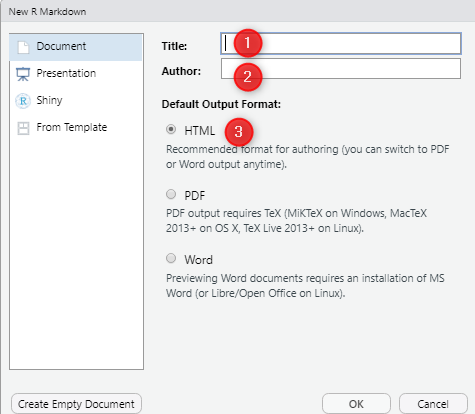
\includegraphics{index_files/mediabag/2.png}

Кроме этих преимуществ есть и много других, о которых мы узнаем в
процессе изучения курса.

\hypertarget{ux43aux43eux435-ux447ux442ux43e-ux435ux449ux435-ux43e-ux440ux430ux437ux440ux430ux431ux43eux442ux447ux438ux43aux430ux445-r}{%
\subsection{Кое-что еще о разработчиках
R}\label{ux43aux43eux435-ux447ux442ux43e-ux435ux449ux435-ux43e-ux440ux430ux437ux440ux430ux431ux43eux442ux447ux438ux43aux430ux445-r}}

Кроме основной команды, в сообществе R выделяются талантливые
программисты, которые разрабатывают библиотеки, без преувеличения
производящие революцию в обработке и анализе данных. Это настоящие гуру,
которых очень уважают в исследовательском сообществе, их имена знают
все, кто работает в R. Ну, или почти все\ldots{}

ТОП-3 (по моему личному мнению)

\begin{enumerate}
\def\labelenumi{\arabic{enumi}.}
\tightlist
\item
  \textbf{Хэдли Уикхэм} (Hadley Wickham) - программист из Новой
  Зеландии, главный научный сотрудник в компании RStudio. Без
  преувеличения самый известнй, очень трудолюбивый и плодотворный
  разработчик R, автор почти 100 (!) библиотек, в том числе таких
  мегапопулярных как \texttt{ggplot}, \texttt{dplyr},
  \texttt{tidyverse}, \texttt{devtools} и других. Этими библиотеками
  воспользовались более 825 тыс. человек.
\end{enumerate}

\includegraphics[width=3.125in,height=\textheight]{index_files/mediabag/hadley.jpg}

\begin{enumerate}
\def\labelenumi{\arabic{enumi}.}
\setcounter{enumi}{1}
\tightlist
\item
  \textbf{Дирк Эддельбуэттель} (Dirk Eddelbuettel) - канадский ученый в
  области статистики, программист и исследователь, второй в нашем списке
  лучших разработчиков библиотек для R. Принял участие в создании более
  60 библиотек, наиболее популярными среди которых является
  \texttt{Rcpp}, позволяющая интегрировать R с другим не менее
  популярным языком C++, а также \texttt{RPostgreSQL}, предоставляющая
  интерфейс для работы с системой баз данных PostgreSQL. Работает в
  Иллинойском университете в Урбане-Шампейне.
\end{enumerate}

\includegraphics[width=3.125in,height=\textheight]{index_files/mediabag/deddel.png.jpg}

\begin{enumerate}
\def\labelenumi{\arabic{enumi}.}
\setcounter{enumi}{2}
\tightlist
\item
  \textbf{Ихуэй Се} (Yihui Xie) - еще один плодовитый разрботчик,
  создавший более 40 библиотек, загруженных более 130 тыс. раз. Его
  большая заслуга в том, что разработал инструменты для создания
  интерактивных приложений (\texttt{knitr}, \texttt{rmarkdown},
  \texttt{shiny} и \texttt{htmlwidgets} - его детища, и мы тоже с ними
  познакомимся на следующих занятиях). Yihui Xie также поддерживает
  систему \texttt{bookdown}, которую можно использовать для написания
  книг и отчетных документов с помощью R Markdown. Инженер-программист
  компании RStudio.
\end{enumerate}

\hypertarget{ux432ux43eux43fux440ux43eux441ux44b-ux434ux43bux44f-ux441ux430ux43cux43eux43fux440ux43eux432ux435ux440ux43aux438}{%
\subsection{Вопросы для
самопроверки**}\label{ux432ux43eux43fux440ux43eux441ux44b-ux434ux43bux44f-ux441ux430ux43cux43eux43fux440ux43eux432ux435ux440ux43aux438}}

\textbf{Каким языком является R?}

\begin{itemize}
\item
  \begin{enumerate}
  \def\labelenumi{(\Alph{enumi})}
  \tightlist
  \item
    компилируемым\\
  \end{enumerate}
\item
  \begin{enumerate}
  \def\labelenumi{(\Alph{enumi})}
  \setcounter{enumi}{1}
  \tightlist
  \item
    процедурным\\
  \end{enumerate}
\item
  \begin{enumerate}
  \def\labelenumi{(\Alph{enumi})}
  \setcounter{enumi}{2}
  \tightlist
  \item
    интерпретируемым\\
  \end{enumerate}
\item
  \begin{enumerate}
  \def\labelenumi{(\Alph{enumi})}
  \setcounter{enumi}{3}
  \tightlist
  \item
    структурным
  \end{enumerate}
\end{itemize}

\textbf{Может ли R быть интегрирована с Hadoop для обработки больших
данных?} TRUE / FALSE

\textbf{На основе какого языка создан R?}

\begin{itemize}
\item
  \begin{enumerate}
  \def\labelenumi{(\Alph{enumi})}
  \tightlist
  \item
    Python\\
  \end{enumerate}
\item
  \begin{enumerate}
  \def\labelenumi{(\Alph{enumi})}
  \setcounter{enumi}{1}
  \tightlist
  \item
    Oracle\\
  \end{enumerate}
\item
  \begin{enumerate}
  \def\labelenumi{(\Alph{enumi})}
  \setcounter{enumi}{2}
  \tightlist
  \item
    S\\
  \end{enumerate}
\item
  \begin{enumerate}
  \def\labelenumi{(\Alph{enumi})}
  \setcounter{enumi}{3}
  \tightlist
  \item
    Java
  \end{enumerate}
\end{itemize}

\bookmarksetup{startatroot}

\hypertarget{ux443ux441ux442ux430ux43dux43eux432ux43aux430-ux438-ux43dux430ux447ux430ux43bux43e-ux440ux430ux431ux43eux442ux44b-ux441-r}{%
\chapter{Установка и начало работы с
R}\label{ux443ux441ux442ux430ux43dux43eux432ux43aux430-ux438-ux43dux430ux447ux430ux43bux43e-ux440ux430ux431ux43eux442ux44b-ux441-r}}

\hypertarget{ux443ux441ux442ux430ux43dux43eux432ux43aux430-r}{%
\section{Установка
R}\label{ux443ux441ux442ux430ux43dux43eux432ux43aux430-r}}

Прежде, чем начать работать с R нам нужно установить его себе на
компьютер. Для этого необходимо перейти по ссылке и выбрать версию,
подходящую для вашей операционной системы (ссылка ниже ведет на версию
для Windows): \url{https://cran.r-project.org/bin/windows/base/}

Вместе с R устанавливается небольшая консоль, в которой можно набирать
команды на R, но работать в ней не очень удобно, поэтому большинство
пользователей предпочитает работать со специальным интерфейсом, или
интегрированной средой разработки. Для языка R создано довольно много
таких сред, однако, наиболее популярной является RStudio.

Это бесплатная программа, скачать которую можно по ссылке.

\url{https://posit.co/products/open-source/rstudio/}

Эти шаги не очень трудны и не потребуют каких-то особых навыков, но на
всякий случай, можно обратиться к однму из обучающих видео:

Как установить R:

\includegraphics{index_files/mediabag/203516510.pdf}

Как установить RStudio:

\includegraphics{index_files/mediabag/203516968.pdf}

В комьютерных классах устанавливать ничего не нужно, эти инструкции для
домашнего использования.

\hypertarget{ux43dux430ux447ux430ux43bux43e-ux440ux430ux431ux43eux442ux44b-ux432-rstudio}{%
\section{Начало работы в
RStudio}\label{ux43dux430ux447ux430ux43bux43e-ux440ux430ux431ux43eux442ux44b-ux432-rstudio}}

После первого запуска RStudio вы, скорее всего, увидите вот такую
картину:

\includegraphics{index_files/mediabag/fig13.jpg}

Основное окно RStudio будет состоять из трех частей (экранов).

Слева находится консоль (Console) - здесь можно писать код, и здесь же
будут появляться результаты его выполнения, а также различные сообщения,
с помощью которых R ``общается'' с пользователями.

Справа сверху - рабочее окружение (Environment) - здесь хранятся
создаваемые и загружаемые объекты - данные (вектора, датафреймы и пр.),
пользовательские функции и некоторые другие объекты. В этом же окне
можно посмотреть историю (History) выполнения кода, и если вы случайно
или специально что-то удалили, часто именно в истории можно найти
строки, которые были выполнены, и их можно восстановить. Здесь есть
некоторые другие вкладки, они нам понадобятся на более поздних этапах
работы с R и RStudio.

Справа снизу - окно просмотра. В отдельных вкладках можно посмотреть,
какие файлы и папки есть в рабочей директории, какие библиотеки
установлены, можно запросить помощь или посмотреть графики (в процессе
анализа).

Это только в первый раз окна всего три.

Выберите в меню File - New File - R Script:


\includegraphics{index_files/mediabag/4.png}

Откроется новый файл, и окон станет четыре:

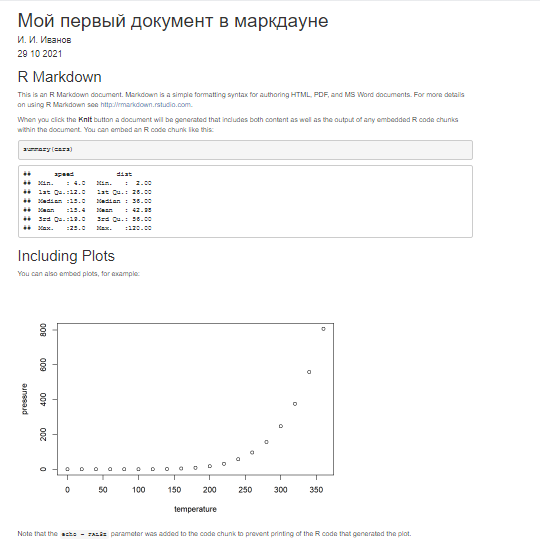
\includegraphics[width=0.8\textwidth,height=\textheight]{index_files/mediabag/5.png}

В этом новом окне можно писать код и комментарии, сохранять его как
отдельный файл с расширением .R, который можно запускать повторно, что
очень удобно и позволяет значительно сохранить время при рутинной
обработке данных. Очень часто в ходе обработки и анализа данных
приходится осуществлять повторяющиеся действия, и скрипт поможет
ускорить процесс обработки. В этом состоит основное отличие от консоли,
где код можно запустить только однажды.

\hypertarget{ux43aux430ux43a-ux443ux441ux442ux430ux43dux43eux432ux438ux442ux44c-ux43dux443ux436ux43dux443ux44e-ux431ux438ux431ux43bux438ux43eux442ux435ux43aux443}{%
\section{Как установить нужную
библиотеку?}\label{ux43aux430ux43a-ux443ux441ux442ux430ux43dux43eux432ux438ux442ux44c-ux43dux443ux436ux43dux443ux44e-ux431ux438ux431ux43bux438ux43eux442ux435ux43aux443}}

Как мы выяснили, базовый язык R в настоящее время используется наряду с
многочисленными функциями и библиотеками, разрабатываемыми коллективами
ученых и разработчиками из разных стран мира, включая Россию.

Устанавливать новые библиотеки нам придется практически на каждом
занятии, поэтому лучше научиться делать это сразу.

Эти библиотеки хранятся в основном в двух местах:

\begin{itemize}
\tightlist
\item
  \href{https://cran.r-project.org/}{CRAN}
\item
  \href{https://github.com/}{Github} - нечто вроде социальной сети для
  программистов, где все друг друга знают, создают совместные проекты и
  делятся кодом.
\end{itemize}

\hypertarget{ux43aux430ux43a-ux443ux441ux442ux430ux43dux43eux432ux438ux442ux44c-ux431ux438ux431ux43bux438ux43eux442ux435ux43aux443-ux441-ux43fux43eux43cux43eux449ux44cux44e-cran}{%
\subsection{Как установить библиотеку с помощью
CRAN}\label{ux43aux430ux43a-ux443ux441ux442ux430ux43dux43eux432ux438ux442ux44c-ux431ux438ux431ux43bux438ux43eux442ux435ux43aux443-ux441-ux43fux43eux43cux43eux449ux44cux44e-cran}}

Чтобы скачать нужную библиотеку (конечно, нужно знать ее название, иначе
ничего не получится) с помощью CRAN, проще всего воспользоваться меню
RStudio:

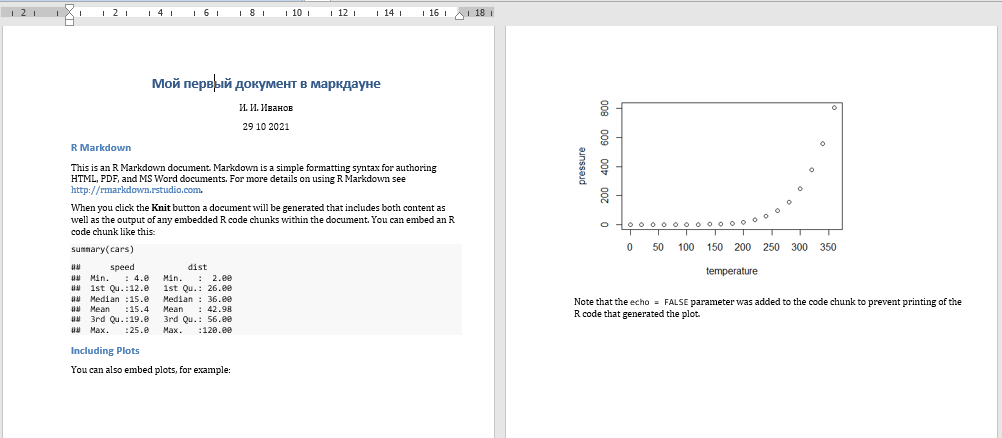
\includegraphics{index_files/mediabag/6.png}

Затем в окне \textbf{Packages} необходимо ввести имя нужной библиотеки и
нажать на кнопку \textbf{Install}.

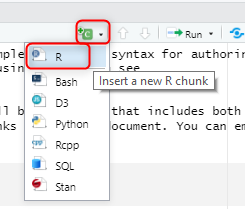
\includegraphics{index_files/mediabag/7.png}

\hypertarget{ux43aux430ux43a-ux443ux441ux442ux430ux43dux43eux432ux438ux442ux44c-ux431ux438ux431ux43bux438ux43eux442ux435ux43aux443-ux438ux437-github}{%
\subsection{Как установить библиотеку из
Github}\label{ux43aux430ux43a-ux443ux441ux442ux430ux43dux43eux432ux438ux442ux44c-ux431ux438ux431ux43bux438ux43eux442ux435ux43aux443-ux438ux437-github}}

Не все библиотеки доступны на CRAN, так как эта процедура достаточно
сложная и строгая, предполагает несколько проверок (кода,
сопроводительной документации). Достаточно частая практика, когда
библиотека еще не подана для регистрации на CRAN, разработчики помещают
ее на GitHub, откуда ее можно скачать и использовать по назначению. Это
позволяет разработчикам получить обратную связь, устранять возможные
ошибки, улучшать код.

\hypertarget{ux43aux43eux435-ux447ux442ux43e-ux43e-ux431ux438ux431ux43bux438ux43eux442ux435ux43aux435ux43fux430ux43aux435ux442ux430ux445}{%
\subsubsection{Кое-что о
библиотеке/пакетах}\label{ux43aux43eux435-ux447ux442ux43e-ux43e-ux431ux438ux431ux43bux438ux43eux442ux435ux43aux435ux43fux430ux43aux435ux442ux430ux445}}

Мы называем ``библиотеку'' ``библиотекой'' и подразумеваем под ней набор
каких-то полезных утилит, потому что так принято в русскоязычном
сегменте Интернета, посвященном программированию.

Однако, по-английски библиотека называется \textbf{package}, то есть
``пакет'', в котором ``упакованы'' функции, сопровождающие документы и
иногда готовые данные, а вот функция, которая этот пакет запускает -
\texttt{library()} - то есть собственно библиотека, такие вот языковый
казус. Об этом стоит помнить и слова эти не путать.

Чтобы установить нужную библиотеку из GitHub, нам понадобится функция
\texttt{install\_github()}, в которой мы должны указать имя разработчика
и название библиотеки. Однако, чтобы выполнить эту функцию, нужна
дополнительная библиотека \texttt{devtools}. Установить ее можно через
CRAN с помощью описанного выше способа. А уже затем, загрузив ее,
установить нужную нам библиотеку (получается сложновато, зато мы сразу
научимся нужным действиям, потом мы доведем их до автоматизма):

\begin{Shaded}
\begin{Highlighting}[]
\FunctionTok{library}\NormalTok{ (devtools)}
\FunctionTok{install\_github}\NormalTok{(}\StringTok{"DeveloperName/PackageName"}\NormalTok{)}
\end{Highlighting}
\end{Shaded}

\hypertarget{ux432ux43eux43fux440ux43eux441ux44b-ux434ux43bux44f-ux441ux430ux43cux43eux43fux440ux43eux432ux435ux440ux43aux438-1}{%
\subsection{Вопросы для
самопроверки}\label{ux432ux43eux43fux440ux43eux441ux44b-ux434ux43bux44f-ux441ux430ux43cux43eux43fux440ux43eux432ux435ux440ux43aux438-1}}

Какой код нужно написать, чтобы подключить для использования библиотеку
\texttt{tidyverse}? r fitb(c(``library( tidyverse )'', ``library(
"tidyverse" )'', ``library( `tidyverse' )''), ignore\_ws = TRUE, width =
``20'')



\end{document}
